%% Nicky Randles - B00058026@Student.itb.ie


\documentclass[12pt,ITBthesis]{report}


\usepackage{amsfonts}
\usepackage{amssymb,amsmath}
\usepackage{amsthm}
\usepackage{newlfont}
\usepackage{graphicx}
\usepackage{tabularx}
\usepackage{longtable}
\usepackage{lscape}
\usepackage{latexsym}
\usepackage{geometry}
\usepackage{fancyhdr}
\usepackage{amsmath}
\usepackage{amsfonts}
\usepackage{amssymb}
\usepackage{subfigure}
\usepackage{times}

\usepackage[hidelinks]{hyperref}


\usepackage{cite}


\begin{document}
	% Fuzz -------------------------------------------------------------------
	\hfuzz2pt % Don't bother to report over-full boxes if over-edge is < 2pt
	% Line spacing -----------------------------------------------------------
	
	\newlength{\defbaselineskip}
	\setlength{\defbaselineskip}{\baselineskip}
	\newcommand{\setlinespacing}[1]%
	{\setlength{\baselineskip}{#1 \defbaselineskip}}
	\newcommand{\doublespacing}{\setlength{\baselineskip}%
		{2.0 \defbaselineskip}}
	\newcommand{\singlespacing}{\setlength{\baselineskip}{\defbaselineskip}}
	% MATH -------------------------------------------------------------------
	\newcommand{\A}{{\cal A}}
	\newcommand{\h}{{\cal H}}
	\newcommand{\s}{{\cal S}}
	\newcommand{\W}{{\cal W}}
	\newcommand{\BH}{\mathbf B(\cal H)}
	\newcommand{\KH}{\cal  K(\cal H)}
	\newcommand{\Real}{\mathbb R}
	\newcommand{\Complex}{\mathbb C}
	\newcommand{\Field}{\mathbb F}
	\newcommand{\RPlus}{[0,\infty)}
	%
	\newcommand{\norm}[1]{\left\Vert#1\right\Vert}
	\newcommand{\essnorm}[1]{\norm{#1}_{\text{\rm\normalshape ess}}}
	\newcommand{\abs}[1]{\left\vert#1\right\vert}
	\newcommand{\set}[1]{\left\{#1\right\}}
	\newcommand{\seq}[1]{\left<#1\right>}
	\newcommand{\eps}{\varepsilon}
	\newcommand{\To}{\longrightarrow}
	\newcommand{\RE}{\operatorname{Re}}
	\newcommand{\IM}{\operatorname{Im}}
	\newcommand{\Poly}{{\cal{P}}(E)}
	\newcommand{\EssD}{{\cal{D}}}
	% THEOREMS ---------------------------------------------------------------
	\theoremstyle{plain}
	\newtheorem{thm}{Theorem}[section]
	\newtheorem{cor}[thm]{Corollary}
	\newtheorem{lem}[thm]{Lemma}
	\newtheorem{prop}[thm]{Proposition}
	%
	\theoremstyle{definition}
	\newtheorem{defn}{Definition}[section]
	%
	\theoremstyle{remark}
	\newtheorem{rem}{Remark}[section]
	%
	\numberwithin{equation}{section}
	\renewcommand{\theequation}{\thesection.\arabic{equation}}
	%%% ----------------------------------------------------------------------
	%%% ----------------------------------------------------------------------
	\makeatletter
	\renewcommand\appendix{%
		\par
		\setcounter{chapter}{0}%
		\setcounter{section}{0}%
		\setcounter{subsection}{0}%
		\gdef\thesection{\@Alph\c@section}
		\gdef\@sect##1##2##3##4##5##6[##7]##8{%
			\refstepcounter{##1}%
			\protected@edef\@svsec{\@seccntformat{##1}\relax}%
			\begingroup
			\hspace{-\parindent}##6\appendixname~ {%
				\@hangfrom{\hskip ##3 \relax\@svsec}\par%
				\hspace{-\parindent}\interlinepenalty \@M ##8 \@@par}%
			\endgroup
			\csname ##1mark\endcsname{##7}%
			\addcontentsline{toc}{##1}{\protect\numberline{\csname the##1\endcsname}##7}%
			\@xsect{##5}%
		}%
	}%
	\makeatother
	
	\setlength{\parskip}{1ex plus 0.5ex minus 0.2ex}
	
	\title{Medical Management Application}
	 
	\author{Nicky Randles - B00058026}
	
	\date{25 October 2015 }
	
	\maketitle
		
	\section{Title:}
	Medical Management Application
	
	\section{Background}
	Technology has really changed the world we live in. It has helped make are lives easier in many ways. It has made it much easier for us to be more organised and communicate with each other. These days many medical practices do not use technology as well as they could to communicate with their patients better. Many medical practises have not been very efficient with the way they assign appointments to patients. Several patients are often given the same appointment time. This can cause appointment rooms to be overcrowded. This can be a health risk to vulnerable patients. It also can be a big inconvenience for others who may be waiting long periods of time. 
	
	 There are similar applications out there which have tried to provide a useful tool for hospitals to make better arrangements for patients. One of the applications I researched was “Book Dr Appointment” \cite{1}. This application has over 90,000 Doctors registered. This application allows new users to join and find a Doctor. They can then book a doctor appointment with the Doctor of their chose. They can then add it to their calendar so they don’t forget when their appointment is scheduled. This application has been quite successful amongst android users. It’s has a 4.5/5 on the Google play store. It has been installed by 5,000 – 10,000 android users. 
	
	Another application which I found during my research was “Doctor Appointment Lite” \cite{2}. Rather than making the appointment with the Doctor through the application, this app only allows the users to store the already scheduled appointment in the app as a reminder. The user can store the appointment in their app and they will receive a notification to remind them of the appointment later. This application also allows users to rate their doctor’s performance. This helps people see who may be a better choice. This app has not been as successful as “Book Dr Appointment”, it received a rating of 3.9/5 on the Google play store and has been downloaded 1,000 -5,000.
	
	\section{Main research questions:}
	\begin{enumerate}
		\item Determine if there is an actual need for an application like this in medical practices.
			\begin{itemize}
				\item I will need to see if there is actual need for the application, if there is not a need for the application it will not be successful.
			\end{itemize}
		\item Determine who the target audiences will be for application like this.
			\begin{itemize}
				\item I will have to find out who the target audience is and work around their specific needs. 
			\end{itemize}
		\item Determine what each target audience will find useful on the application.
			\begin{itemize}
				\item If there is more than one target audience I will have to see what parts of the application each will find useful.
			\end{itemize}
		\item How will it compare to existing applications already available to the market.
			\begin{itemize}
				\item I will have to research other applications and see what they bring to the table. I will have to make an application better than theirs for it to be successful.
			\end{itemize}
		\item Decide on what approach to take to make the application as user friendly as possible.
			\begin{itemize}
				\item I need to look into the different designs out there and see which ones are liked more amongst the users of similar applications
			\end{itemize}
	\end{enumerate}
	
	\section{Justification/Benefits:}
	This application will be very helpful for everyone who uses it. It will be helpful for both the doctors and patients. It will provide doctors with the ability to arrange their patient’s appointments in a more efficient way. This application will help them get the most possible out of their time. This application will help patients increase their chances of being seen at their scheduled time than before. They shouldn’t have to waste as much time waiting to see their doctor. This application will also help patients stay more organised. Their appointments will be stored in their calendar and they will be reminded when their appointments are. This application will also help decrease overcrowding as patients will not be double booked through this app. 
	
	It can help increase the satisfaction patients have with their doctors. As we all know waiting for a doctor can be a very anxious time. The patient may be worried about the appointment or possibly in pain. In a study by Press Ganey, they discovered that the average waiting time for a patient was 24 minute in 2009 \cite{3}. I personally believe that it has probably increased even higher now. This application will help lower these waiting times for patients.
	
	\section{Feasibility:}
	After carrying out some research on the different aspects of this application, I am very confident that it is technically feasible. Over the last few years I have gained a good understanding of Android, HTML, CSS, PHP, XML, and MYSQL. I’m am confident that I will have the ability to complete all of the tasks involved in this application with what I have learned so far. The supervisor of this project is very knowledgeable of these areas too and will be able to keep the application development going in the right direction. By planning out the different tasks involved in this project I should be able to complete it in the allocated time frame.
	
	\section{Proposed Methodologies:}
	I will be taking an adaptive approach to this project as it is more flexible because it assumes the project cannot be completely planned out in advance. The Software Development Life Cycle model I think is best suited for this project is the Spiral model. I think it is the best SDLC for this project as it involves a lot of testing which will help me to end up with a better final product 
	The spiral model is similar to the waterfall model but it is an upgraded version. The spiral model consists of four phases. They are Planning, Risk Analysis, Engineering and Evaluation. A software project will go through these phases in iteration. This approach assumes that no one gets it right the first time, each iteration refines the previous result.
	
	\begin{itemize}
		\item Planning Phase: In this phase requirements and objectives are gathered 
		\item Risk Analysis Phase: In this phase risks are identified and are analysed. Alternative solutions are also evaluated.
		\item Engineering Phase: In this phase the software is developed and testing is carried out. 
		\item Evaluation Phase: In this phase the user is able to evaluate the project output so far before it takes its next spiral. 
	\end{itemize}
	
	The main advantage of the spiral model is that it reduces the chances of project failure. This is achieved through extensive risk analysis. By carrying out risk analysis it can help avoid risks which could cause the project to fail.
	
	\begin{figure}[!h]
		\centering
		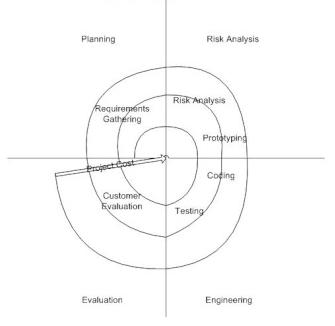
\includegraphics[width=0.4\textwidth]{spiralModel}
		\label{ft_fig_firstfig}
		\caption{Spiral Model \cite{4}}
	\end{figure}
	
	\section{Expected results:}
	The main outcome of this project will be to create an application that can be used by both doctors and patients to arrange appointments. This application should improve the relationship doctors and patients share. The doctors should be able to arrange their appointments better so that patients do not have to wait on the doctors as long. The application should help doctors avoid double bookings and overcrowding in their waiting rooms. It should also help patients be more organised and aware of their upcoming appointments. The application should provide users with a calendar to show their upcoming appointments and should remind them when their appointments are. The application should help improve patient’s satisfaction and decrease issues with doctors and patients.
	
	\section{Conclusion:}
	I plan on carrying out further research into existing applications which deal with scheduling appointments between doctors and their patients. I plan on researching them mainly so that I can see what they do right and what they wrong. I hope to improve on their mistakes and make an application which is more beneficial to the users. Based on the information shown in this project proposal it has been agreed that this project is feasible. This project is now ready to be started. The next step to take is to research available sources in depth.
	
	\setlinespacing{1.0}
	\renewcommand*{\bibname}{\section{References}}
	\bibliographystyle{plain}
	\bibliography{bibliography}
	   
	\section{Project plan:}
	\begin{table}[!h]
		\centering
		\label{my-label}
		\begin{tabular}{l|l|p{8cm}}
		\hline
		1 & Project Proposal & A document that contains information about the project and task that need to be completed.\\ \hline
		2 & Research on similar application & Research on existing applications that involve scheduling appointments.\\ \hline
		3 & Literature Review & An evaluative report on the information found in the literature relating to patient scheduling. \\ \hline
		4 & Risk analysis & Analyse the risk involved in taking on this project.\\ \hline
		5 & Cost assessment & Analyse the potential cost of the project.\\ \hline
		6 & Application design & Start designing the application. Conduct wire framing.\\ \hline
		7 & Develop application & Start developing the application with the necessary resources.\\ \hline
		8 & Application testing & Test the application to discover any existing problems.\\ \hline
		9 & Document results & Document findings during testing process.\\ \hline
		10 & Final application & Fix any problems in application and get working 100 percent.\\ \hline
		11 & Documentation & Put all documents together. Finish off thesis.\\
		12 & Prepare presentation & Prepare for presentation through notes and slides.
		\end{tabular}
		\caption{Work breakdown structure}
	\end{table}
	
	\begin{figure}[!h]
		\centering
		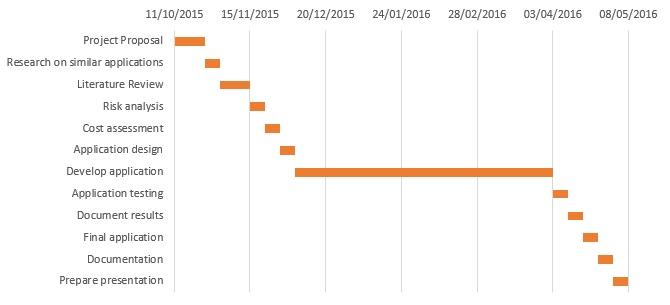
\includegraphics[width=1\textwidth]{ganttChart}
		\label{ft_fig_firstfig}
		\caption{Gantt Chart} 
	\end{figure}

\end{document}

